% THIS IS SIGPROC-SP.TEX - VERSION 3.1
% WORKS WITH V3.2SP OF ACM_PROC_ARTICLE-SP.CLS
% APRIL 2009
%
% It is an example file showing how to use the 'acm_proc_article-sp.cls' V3.2SP
% LaTeX2e document class file for Conference Proceedings submissions.
% ----------------------------------------------------------------------------------------------------------------
% This .tex file (and associated .cls V3.2SP) *DOES NOT* produce:
%       1) The Permission Statement
%       2) The Conference (location) Info information
%       3) The Copyright Line with ACM data
%       4) Page numbering
% ---------------------------------------------------------------------------------------------------------------
% It is an example which *does* use the .bib file (from which the .bbl file
% is produced).
% REMEMBER HOWEVER: After having produced the .bbl file,
% and prior to final submission,
% you need to 'insert'  your .bbl file into your source .tex file so as to provide
% ONE 'self-contained' source file.
%
% Questions regarding SIGS should be sent to
% Adrienne Griscti ---> griscti@acm.org
%
% Questions/suggestions regarding the guidelines, .tex and .cls files, etc. to
% Gerald Murray ---> murray@hq.acm.org
%
% For tracking purposes - this is V3.1SP - APRIL 2009

\documentclass{acm_proc_article-sp}

\begin{document}

\title{A Sample {\ttlit ACM} SIG Proceedings Paper in LaTeX}
\subtitle{[Extended Abstract]}

\numberofauthors{4} 
\author{
\alignauthor
Author One\titlenote{Now on postdoctoral fellow at ABC University}\\
       \affaddr{Institute One}\\
       \affaddr{Address One}\\
       \email{author.one@emails.com}
\alignauthor
Author Two\\
       \affaddr{Institute Two}\\
       \affaddr{Address Two}\\
       \email{author.two@emails.com}
\and % go to new row
\alignauthor
Author Three\\
       \affaddr{Institute Three}\\
       \affaddr{Address Three}\\
       \email{author.three@emails.com}
\alignauthor
Author Four\\
       \affaddr{Institute Four}\\
       \affaddr{Address Four}\\
       \email{author.four@emails.com}
}

\date{20 April 2013}


\maketitle
\begin{abstract}
Consumer reviews of restaurants are scattered across various websites in the Internet. A typical user, on an average, visits more than two such websites to get the reviews of the restaurant in question. He also spends a considerable amount of time to get an overall idea of the quality of the restaurant by manually comparing the reviews in those websites. On the other hand, users who visit just one or two sites are not satisfied with the quality of the reviews and are often misled by the ratings. In order to gain insights into the problem, we conducted an online survey with a set of relevant questions and collected the opinion of various users. In this paper,we discuss the data collection methods employed and how it helped us to identify the problems faced by the users. A sample solution could be an online tool that aggregates the reviews from multiple websites and presents the information to the user by normalizing the ratings. Such a tool will save the time and the efforts taken by the users in getting the reviews and provide a hassle-free option to get the aggregated reviews from the most popular websites.

\end{abstract}

% A category with the (minimum) three required fields
\category{H.4}{Information Systems Applications}{Miscellaneous}
%A category including the fourth, optional field follows...
\category{D.2.8}{Software Engineering}{Metrics}[complexity measures, performance measures]

\terms{Theory}

\keywords{ACM proceedings, \LaTeX, text tagging} % NOT required for Proceedings

\section{Introduction}
Sample text. Sample text. Sample text. Sample text. Sample text. Sample text. 
Sample text. Sample text. Sample text. Sample text. Sample text. Sample text. 
Sample text. Sample text. Sample text. Sample text. Sample text. Sample text. 
Sample text. Sample text. Sample text. Sample text. Sample text. Sample text. 
Sample text. Sample text. Sample text. Sample text. Sample text. Sample text. 
Sample text. Sample text. Sample text. Sample text. Sample text. Sample text. 
Sample text. Sample text. Sample text. Sample text. Sample text. Sample text. 

Citation of Einstein paper~\cite{Einstein}.

\section{Survey Results and Discussions}
To have a detailed idea about our problem statement and to establish the requirement for a solution we conducted a survey with a set of 9 questions. These questions were mainly focused on the usage patterns of the participants and the problems they experienced while selecting a restaurant to visit. The survey had nearly a hundred participants and it ensured the anonymity of the participants to ensure their unbiased responses.

\begin{figure}[htp]
\centering
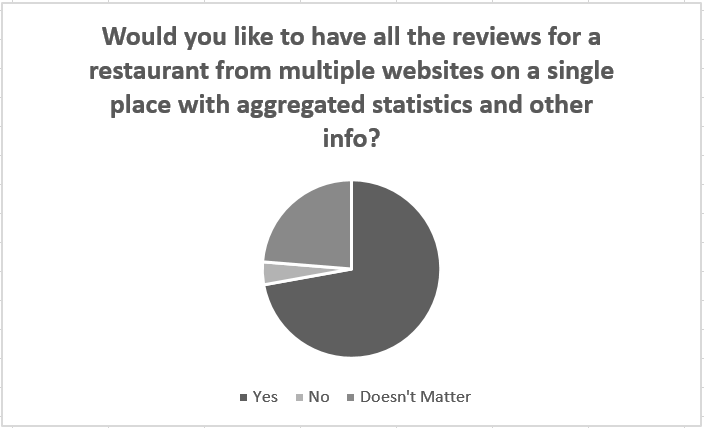
\includegraphics[width=8.5cm]{need_web}
\caption{Question 1}
\label{fig:question1}
\end{figure}

Lorem ipsum dolor sit amet, consectetur adipiscing elit, sed do eiusmod tempor incididunt ut labore et dolore magna aliqua. Ut enim ad minim veniam, quis nostrud exercitation ullamco laboris nisi ut aliquip ex ea commodo consequat. Duis aute irure dolor in reprehenderit in voluptate velit esse cillum dolore eu fugiat nulla pariatur. Excepteur sint occaecat cupidatat non proident, sunt in culpa qui officia deserunt mollit anim id est laborum.

Lorem ipsum dolor sit amet, consectetur adipiscing elit, sed do eiusmod tempor incididunt ut labore et dolore magna aliqua. Ut enim ad minim veniam, quis nostrud exercitation ullamco laboris nisi ut aliquip ex ea commodo consequat. Duis aute irure dolor in reprehenderit in voluptate velit esse cillum dolore eu fugiat nulla pariatur. Excepteur sint occaecat cupidatat non proident, sunt in culpa qui officia deserunt mollit anim id est laborum.

Lorem ipsum dolor sit amet, consectetur adipiscing elit, sed do eiusmod tempor incididunt ut labore et dolore magna aliqua. Ut enim ad minim veniam, quis nostrud exercitation ullamco laboris nisi ut aliquip ex ea commodo consequat. Duis aute irure dolor in reprehenderit in voluptate velit esse cillum dolore eu fugiat nulla pariatur. Excepteur sint occaecat cupidatat non proident, sunt in culpa qui officia deserunt mollit anim id est laborum.

\section{Conclusion}
The survey has been conducted with a predefined set of questions and the responses from various users has been plotted graphically for further analysis. The results of the survey convince us that the users do face problems when they try to gather reviews for a restaurant. Some of the users are not satisfied with the quality of the reviews while others spend sometime visiting multiple sites to cross verify the reviews. Hence they need a better tool which would solve their problem and save their time. We have a couple of solutions in mind and one of which is aggregating the reviews from multiple sites and we are planning to pick the top websites that are rated by the users in our survey. This would convince the users that our aggregated results are from a reliable source and provide a better view of the quality of the restaurant. 


\bibliographystyle{abbrv}
\bibliography{sample}

%\balancecolumns 

\end{document}
